\author {Перминова Виктория}
\title{Лабораторная работа 3}

\documentclass[10pt]{article}
\usepackage[T2A]{fontenc}
\usepackage[russian]{babel}
\usepackage{multicol}
\usepackage{enumitem}
\usepackage{graphicx}
\usepackage[top=2cm, bottom=2cm, left=1.6cm, right=1.6cm, footskip=15mm]{geometry}
\makeatletter
\renewcommand{\fnum@figure}{Figure \thefigure}
\makeatother
\bibliographystyle{unsrt}
\setlist[enumerate]{itemsep=0pt, parsep=0pt, partopsep=0pt, topsep=0pt}
\setlength\parindent{15pt}
\setlength{\columnsep}{0.5cm}
\pagenumbering{arabic}
\setcounter{page}{60}



\begin{document}
{\begin{multicols*}{2}
\begin{enumerate}
\fontfamily{ptm}\selectfont\footnotesize
\item [{[66]}] {R. Serdyukov, “Bazovye algoritmy i instrumental’nye sredstva
obrabotki informacii v grafodinamicheskih associativnyh mashinah
[Basic algorithms and tools for information processing in
graphodynamic associative machines],”  PhD  diss.: 05.13.11,
Minsk,  2004,  114 p} 
\item [{[67]}] {V. Golenkov, N. Gulyakina, and D. Shunkevich, \textit{Standart otkrytoj
tekhnologii ontologicheskogo proektirovaniya, proizvodstva i
ekspluatacii semanticheski sovmestimyh gibridnyh intellektual’nyh
komp’yuternyh sistem [Standard of the open technology for
ontological design, production, and operation of semantically
compatible hybrid intelligent computer systems]}, V. Golenkov, Ed.
Minsk: Bestprint, 2021.} 
\item [{[68]}] {J. von Neumann, \textit {Teoriya samovosproizvodyashchihsya avtomatov [Theory of self-reproducing automata]}. M.: Mir, 1971, (In Russ.).} 
\item [{[69]}] {D.A. Moon, “Symbolics architecture,” \textit{ Computer}, vol. 20, no. 1, pp.
43–52, 1987. [Online]. Available: doi:10.1109/MC.1987.1663356} 
\item [{[70]}] {S. Smith, “The LMI Lambda Technical Summary. Technical report,
LMI Inc.” Los Angeles, CA, 1984.}  
\item [{[71]}] {G. L. Steele and W. D. Hillis, “Connection Machine Lisp: finegrained parallel symbolic processing,” in \textit{Proceedings of the 1986
ACM conference on LISP and functional programming (LFP ’86).}
New York: ACM, 1986, pp. 279–297.} 
\item [{[72]}] {P. McJones. (2018, Dec.) Parallel Lisps: Connection Machine Lisp (StarLisp). Computer History Museum. Mode of access:
https://www.softwarepreservation.org/projects/LISP/parallel\#\\Connection\_Machine\_\textbackslash protect\textbackslash discretionary{\textbackslash protect\textbackslash protect\textbackslash
\\leavevmode@ifvmode\textbackslash kern+.1667em\textbackslash relax\textbackslash OMS/cmsy/m/n/8\textbackslash
\\char2}{}{}Lisp\_(StarLisp). - Date of access: 29.12.2018.}
\item[{[73]}] {V. van der Leun, \textit{Introduction to JVM Languages}. Packt
Publishing, Jun. 2017.} 
\item[{[74]}] {V. Ivashenko, “String processing model for knowledge-driven
systems,” \textit{Doklady BGUIR}, vol. 18, pp. 33–40, 10 2020.}
\item[{[75]}]{B. Rasheed and A. Popov, “Network Graph Datastore Using
DISC Processor,” in \textit{2019 IEEE Conference of Russian Young
Researchers in Electrical and Electronic Engineering (EIConRus)},
Jan. 2019, pp. 1582–1587.} 
\item[{[76]}] {E. Dubrovin and A. Popov, “Graph representation methods for
the discrete mathematics instructions set computer,” in \textit{2020
IEEE Conference of Russian Young Researchers in Electrical and
Electronic Engineering (EIConRus)}, Jan. 2020, pp. 1925–1930.}
\item[{[77]}]{C. Hewitt. Middle History of Logic Programming: Resolution,
Planner, Prolog and the Japanese Fifth Generation Project.\\
Mode of access: http://citeseerx.ist.psu.edu/viewdoc/download;\\
jsessionid=07A4074D9BBEC56C92085D21A10A6B4D?doi=10.
1.1.363.\&rep=rep1\&type=pdf. — Date of access: accessed
20.03.2020.
}
\item[{[78]}]{V. Ivashenko, \textit{Modeli resheniya zadach v intellektual’nyh sistemah.
V 2 ch. CH. 1 : Formal’nye modeli obrabotki informacii i
parallel’nye modeli resheniya zadach : ucheb.-metod. posobie
[Problem-solving models in intelligent systems. In 2 p. P. 1 :
Formal models of information processing and parallel problem\-solving models: study guide]}. Minsk: BSUIR, 2020, (In Russ.).}
\item[{[79]}]{“LegUp High-Level Synthesis,” mode of access: http://legup.eecg.
utoronto.ca/. — Date of access: 29.03.2023.} 
\item[{[80]}]{“VHDPlus,” mode of access: https://vhdplus.com/. — Date of
access: 29.03.2023.}
\item[{[81]}]{“SystemC Community Portal,” mode of access: https://systemc.
org/. — Date of access: 29.03.2023.}
\item[{[82]}]{“MyHDL,” mode of access: https://www.myhdl.org/. — Date of
access: 29.03.2023.} 
\item[{[83]}]{P. Sapaty, \textit{“Yazyk VOLNA-0 kak osnova navigacionnyh struktur
dlya baz znanij na osnove semanticheskih setej [language VOLNA-0 as the basis of navigation structures for knowledge bases based
on semantic networks],” Iss. of the USSR Academy of Sciences.
Technical cybernetics}, no. 5, pp. 198–210, 1986.} 
\item[{[84]}]{D. I. Moldovan and Y.-W. Tung, “SNAP: A VLSI architecture
for artificial intelligence processing,” \textit{Journal of Parallel and
Distributed Computing}, vol. 2, no. 2, pp. 109–131, 1985.
[Online]. Available: https://www.sciencedirect.com/science/article/
pii/0743731585900310} 
\item[{[85]}]{A. Letichevsky, Yu. Kapitonova, V. Volkov, V. Vyshemirsky, and
A. Letichevsky (j.), “Insercionnoe programmirovanie [Insertion
programming],” \textit{Kibernetika i sistemnyj analiz [Cybernetics and
system analysis}], no. 1, pp. 19–32, 2003.} 
\item[{[86]}]{A. Letichevsky, “Insercionnoe modelirovanie [Insertion modeling],”\textit{ Upravlyayushchie sistemy i mashiny [Control systems and
machines}], no. 6, pp. 3–14, 2012.} 
\item[{[87]}]{J. Backus, “Can programming be liberated from the von Neumann
style?” \textit{Communications of the ACM}, vol. 21, no. 8, pp. 613–641,
Aug. 1978. [Online]. Available: https://doi.org/10.1145/359576.
359579} 
\item[{[88]}]{V. Kotov and A. Nariniani, “Asinhronnye vychislitel’nye processy
nad obshchej pamyat’yu [Asynchronous computing processes over
shared memory],” \textit{Kibernetika [Cybernetics]}, no. 3, pp. 64–71,
1966.} 
\end{enumerate}
\begin{center}
\subsection*{Ассоциативные семантические
компьютеры для интеллектуальных
компьютерных систем нового поколения}
\Large Голенков В. В., Шункевич Д. В.,
Гулякина Н. А., Ивашенко В. П.,
Захарьев В. А
\end{center}

В работе рассмотрены недостатки доминирующей
в настоящее время фон-Неймановской архитектуры
компьютерных систем в качестве основы для построения интеллектуальных компьютерных систем нового
поколения, проведен анализ современных подходов
к разработке аппаратных архитектур, устраняющих
некоторые из указанных недостатков, обоснована
необходимость разработки принципиально новых аппаратных архитектур, представляющих собой аппаратный
вариант реализации платформы интерпретации систем,
построенных на базе Технологии OSTIS, — \textit{ассоциативных семантических компьютеров}.

Предложены общие принципы, лежащие в основе \textit{ассоциативных семантических компьютеров}, рассмотрены три возможных варианта архитектуры таких компьютеров, представлены их достоинства и недостатки.
\vspace{5pt}
\begin{flushright}
Received 13.03.2023
\end{flushright}
\end{multicols*}

\clearpage
\begin{center}
    \section*{\Huge Open Semantic Technology as the Foundation
for New Generation Intelligent Systems}
\vspace{13pt}
Mikhail Tatur and Anton Paramonov\\
\textit{Belarusian State University of Informatics and Radioelectronics}\\
Minsk, Republic of Belarus\\
tatur@bsuir.by, a.paramonov@bsuir.by
\vspace{12pt}
\end{center}

\begin{multicols*}{2}
\textbf{\textit{Abstract}—Issues of new generation intelligent 
systems development are discussed. A hypothesis is proposed: for 
the effective implementation of the OSTIS Ecosystem project,
it is necessary to create a fundamentally new computer
architecture (specialized computers)..}

\textbf{\textit{Keywords}—OSTIS technology, Ecosystem, Intelligent
Systems, Specialized computers, Hardware Platform}
\vspace{10pt}
\begin{center}
  {\large I. I}NTRODUCTION  
\end{center}

Artificial Intelligence, like any young scientific direction, develops in leaps and bounds, replacing one
generation of technical systems with others. Let’s try to
present an condition ontology of this direction, which
reflects the subjective vision of the authors.

\textit{We will make a reservation right away that in this
article we will try to use generally accepted statements
and trends to avoid unnecessary controversy. We will
use the generally accepted understanding of Artificial
Intelligence, which stages of evolution are distinguished,
at what stage of progress we are now, etc.}

We will consider an intelligent system as a product
obtained as a result of mathematical apparatus applying, developing algorithms and software and hardware
implementation without specifying the application. The
mnemonic scheme of the intelligent systems ontology
can be represented as three components, as shown in
Fig.1. It‘s no coincidence that in the figure the Mathematical Model (as a paradigm, in a broader sense) intersects
with the Algorithms that implement it, and the Hardware
Platform intersects with the Software.

In most cases, when creating intelligent systems, they
use the mathematical apparatus of Neural Networks
and Machine Learning - in Data Processing, as well
as Semantic Networks, Inference and Ontologies – in
Knowledge Processing (Knowledge Discovery). In addition, Evolutionary Design and Fuzzy Sets are used
as extended tools for these paradigms to increase the
efficiency of solving intellectual problems.

\textit{\underline{Remark.} In the context of this work, we will not refer
to the role of Linguistics, Neurophysiology, and other
fundamental disciplines. They, of course, influenced both
the formation of Artificial Intelligence, and still influence
its development, but are not the topic of the current
discussion.}

For each mathematical direction, there is a wide range
of technological software support to creating intelligence
applications (Tensor Flow, Coffee, ScikitLearn Python,
Keras, R, etc.). The hardware platform is traditionally
presented as “universal” and “specialized”. The universal platform includes conventional computers with
GPUs, as well as supercomputers and computing clusters.
A specialized platform is mainly neurocomputers and
graphic computers (semantic, associative). It‘s easy to
see that specialized “intelligent” computers correspond to
the main artificial intelligence mathematical paradigms.
If we trace the development chronology of this area
of hardware platforms, we will notice obvious surges
and falls in the interest of the scientific community
and developers. You can also note a wide variety of
architectures and technical solutions proposed at different
times \cite{first} \cite{second} \cite{third}

\vspace{10pt}
As an example, we can highlight one of the latest
developments announced by the Moscow State Technical
University named after N. E. Bauman – “Leonhard” [4].
As the author’s state: “ ... for the first time in the history
of computing, a universal computing system with many
instruction streams and one data stream (MISD) has been
developed that implements the DISC (Discrete Mathematics Instruction Set computer) instruction set.” There
have been quite a few such statements in the past, but
none of the specialized «intelligent computers» has found
mass industrial use. In our opinion, this is explained by
the simple victory of “universal” computers in competition with specialized processors. As a rule, intelligent
computing algorithms are highly complex, and therefore
require the appropriate performance of the hardware
platform. Therefore, throughout the development of the
intelligent computing direction, there have been periodic
attempts to create specialized (problem-oriented) architectures, the so-called. neurocomputers, graphic computers, semantic computers, associative computers, focused
on supporting the corresponding computing paradigm.
However, over and over again, special processors were
inferior in their characteristics to modern “universal”
(multi-core and graphics) computers. In particular, the
narrow application focus of specialized computers with
large (even huge) development costs in terms of time and
\end{multicols*}
\begin{figure}
    \centering
    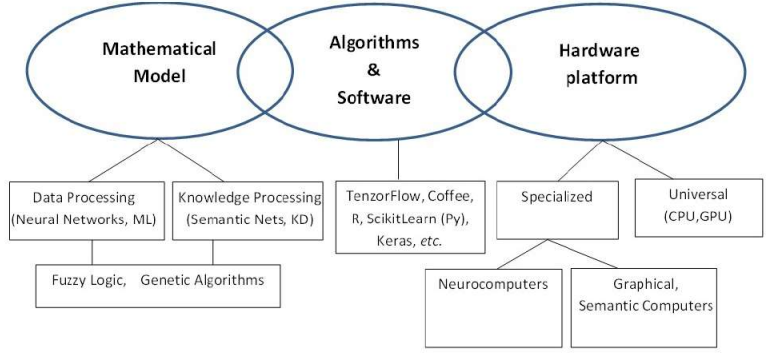
\includegraphics[width=0.98\textwidth]{ontology.png}
    \caption{Ontology of intelligent systems}
\end{figure}
\begin{multicols*}{2}
\noindent price offset the expected performance gain. In addition,
general electronic technologies consistently improve the
performance of «universal» computers. In general, a
paradoxical situation has occurred in the Artificial Intelligence field. On the one hand, there is the possibility of a
quick and relatively inexpensive (using existing libraries
and universal software and hardware platforms) creation
of highly specialized, commercially successful products
with a formal manifestation of intellectual properties.
On the other hand, this hinders the development of
new (FUNDAMENTALLY NEW) intelligent systems
with qualitatively new properties and higher technical
characteristics.

The purpose of this presentation is to reflect on what
it could be like a New Generation of Intelligent Systems,
and what impact OSTIS will have in its emergence.
\vspace{10pt}
\begin{center}
  {\large II. G}ENERAL TREND IN THE DEVELOPMENT OF
{\large A}RTIFICIAL {\large I}NTELLIGENCE TECHNOLOGIES
 \end{center}
 
As a result of a series of industrial and information
revolutions, society has moved into a qualitatively new
stage of its evolution. Now the information sector occupies a decisive and important position in the context
of the development of fundamentally new information
technologies aimed at acquiring, processing, and storing knowledge. Currently, UNESCO is promoting the
concept of the knowledge society as an antithesis of
the concept of the Information Society, the success of
which depends primarily on the development of the
knowledge-based economy [5]. The indicated trends inevitably lead to digitalization, automation, and finally
Digital Transformation of current business processes. It‘s
important to highlight that the use of Artificial Intelligence technologies is one of the fundamental principles
of the society digital transformation [6]. Today we can
state certain successes and practical achievements in
the implementation of commercially successful projects
of intelligent computer systems. However, despite the
apparent prospects, it can be assumed that with the
development of the information society (with a further
increase in the volume of information), the approaches
underlying such systems will reach the limit of their capabilities, just as it happened before with many computer
systems for data processing. Combining many intelligent
services into Digital Platforms significantly increases the
efficiency of solving a particular range of tasks. This
is achieved by Distributing Computations and powers
between resources that are available within the platform
to all its participants (Fig. 2). The use of an architecture based on autonomous services (also known as
Microservices) allows you to speed up the development
process and organize the formation of various platform
configurations. At the same time, the Knowledge Base
of each such service is built autonomously and is often
encapsulated within its implementation. This gives rise
to multiple duplication of information and redundancy in
the knowledge processing. In this connection, it should
be noted that the problematic issues of metadata and
ontologies of the modern information society are strongly
connected with the problems of "conceptual plurality of
information" and "data representation in subject areas of
knowledge".
\vspace{5pt}

However, the most promising approach to building AI
applications is the collaboration of intelligent systems,
which forms a single complete ecosystem. This solution is projected to solve a wide class of problems in various
\end{multicols*}

\clearpage

\bibliography{list}
}
\end{document}